%!TEX TS-program = xelatex

%%%%%%%%%%%%%%%%%%%%%%%%%%%%%%%%%%%%%%%%%%%%%%%%
% CV template
% Originally created by Adrien Friggeri
% Improved by Carmine Benedetto
%%%%%%%%%%%%%%%%%%%%%%%%%%%%%%%%%%%%%%%%%%%%%%%%
%\newcommand\equalhat{\mathrel{\stackon[1.5pt]{=}{\stretchto{%
 %%   \scalerel*[\widthof{=}]{\wedge}{\rule{1ex}{3ex}}}{0.5ex}}}}
%%%
\documentclass[a4paper]{cv-class}
\usepackage[german]{babel}
\usepackage{fontspec}
%\setmainfont[Ligatures = TeX]{TeX Gyre Pagella}

\usepackage{afterpage}
\usepackage{hyperref}
\usepackage{color}
\usepackage{xcolor}
\hypersetup{
    colorlinks=true,
    linkcolor=blue
}
%%%
\usepackage{marvosym}

\addbibresource{bibliography.bib}
\RequirePackage{xcolor}
\definecolor{pblue}{HTML}{0395DE}
%%%% tamaño graficos
\usepackage[export]{adjustbox}% http://ctan.org/pkg/adjustbox
% Resize figures that are too wide for the page.
\let\oldincludegraphics\includegraphics
\renewcommand\includegraphics[2][]{%
  \oldincludegraphics[#1,max width=10cm,max height=\textheight]{#2}
}
%%%



\begin{document}
\header{\qquad Juan Carlos}{~Chavarr\'ia}
      {Mathematiker \& Data Scientist}

% Fake text to add separator
\vspace{1.0cm}
\fcolorbox{white}{gray}{\parbox{\dimexpr\textwidth-2\fboxsep-2\fboxrule}{%
.....
}}

% In the aside, each new line forces a line break
\begin{aside}
  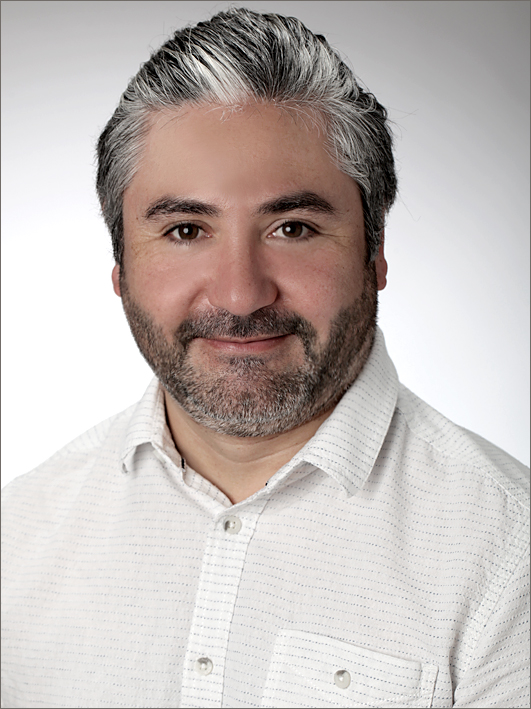
\includegraphics[scale=0.8]{foto_chavarria.jpg}
  	~
  \section{Adresse}
    Wilhelm-Leuschner-Str. 6A \\
    33615 Bielefeld
    ~
  \section{Telefon}
    0177/3804995
    ~
  \section{Mail}
  \underline{\href{mailto:chavarriam.juancarlos@gmail.com}{\footnotesize{chavarriam.juancarlos@gmail.com}}}
 % \\ \vspace{11pt}
 % \underline{\href{mailto:juan.chavarria@uni-bielefeld.de}{\footnotesize{juan.chavarria@uni-bielefeld.de}}}
   ~
  \section{Git}
  	\underline{\href{https://github.com/JuanCaChavaMor}{\footnotesize{github.com/juancachavamor}}}
   % \underline{\href{https://no.linkedin.com/in/martinothamar}{linkedin.com/in/martinothamar}}
   % \underline{\href{https://github.com/martinothamar}{github.com/martinothamar}}
   % ~
  % \section{Preferencia de OS}
  %  \asidelist{\textbf{Linux}}
   % {
\includegraphics[scale=0.30]{img/star.png}
    %
\includegraphics[scale=0.30]{img/star.png}
 %   
\includegraphics[scale=0.30]{img/star.png}
  %  
\includegraphics[scale=0.30]{img/star.png}
   % 
\includegraphics[scale=0.30]{img/star.png}}
  %  \asidelist{\textbf{Windows}}
   % {
\includegraphics[scale=0.30]{img/star.png}
   % 
\includegraphics[scale=0.30]{img/star.png}
  %  
\includegraphics[scale=0.30]{img/star.png}
  %  
\includegraphics[scale=0.30]{img/star.png}
  %  
\includegraphics[scale=0.30]{img/star_empty.png}}
    ~
    %\begin{aside}
%\vspace{0.0cm}
  %\section{Places lived}
  %  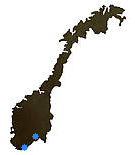
\includegraphics[scale=0.62]{img/norway.png}
   \section{Persönliche Kompetenzen}
 
  \hspace{-.8cm}
        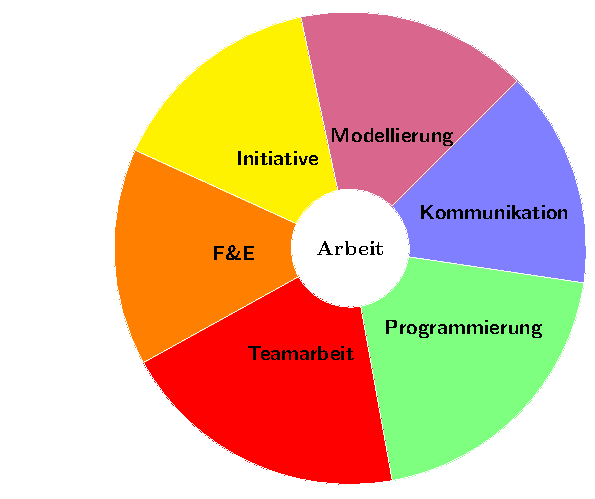
\includegraphics[width=\textwidth,height=\textheight,keepaspectratio]{img/arbeit-cv.pdf}
   ~
  
%   \section{Computerkenntnisse}
%   
%   \hspace{-.8cm}
%     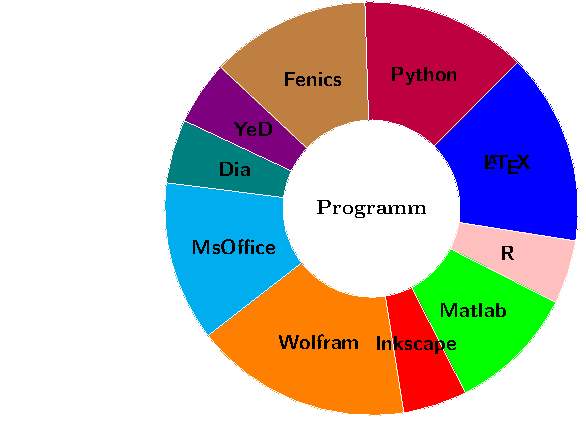
\includegraphics[width=\textwidth,height=\textheight,keepaspectratio]{img/software.pdf} 
%   
%     ~
%\end{aside}
\end{aside}

\vspace{0.5cm}
 %\newpage

\section{Berufserfahrung}
\begin{entrylist}
\entry
{06.2022 - 07.2023}{Mitarbeiter}{Combi Verbrauchermarkt
Einkaufsstätte GmbH \& Co. KG}{Teilzeitjob im Lager und an der Kasse}
\entry
{07.2020}{Vorbereitungslehrer Mathematik}{Bibis - Bildungswerk des
Bielefelder Schulvereins}{Vorbereitung auf die Aufnahmeprüfung
am Studienkolleg}
\entry
{03.2020 - 02.2022}{Honorarlehrkraft} {Nachhilfe Schomberg, Bielefeld}{Nachhilfelehrer für Mathematik und Physik}
\entry
{12.2018 - 09.2019\!}{Wissenschaftlicher Mitarbeiter}{Classroommate SPA, Santiago, Chile}{Statistische Auswertung der Effizienz einer Lernplattform}
\entry
    {10.2018 - 02.2019}
    {Pädagogischer Mitarbeiter}
    {Tecnologías del Sur Sociedad Limitada, Santiago, Chile}
    {Entwicklung von Lehrmaterialien für Energieeffizienzschulungen für kleine und mittlere Unternehmen, finanziert vom chilenischen Energieministerium}
\entry
    {2005 - 2018}
    {Wissenschaftlicher Mitarbeiter}
    {Technische Universität Federico Santa María (UTFSM), Valpara\'iso, Chile}
    {Lehrkraft für Mathematik-Kurse: Differential- und Integralrechnung in einer und mehreren Variablen; lineare Algebra; Fourier Analysis; Vektor Analysis; gewöhnliche und partielle Differentialgleichungen}
 \entry
    {2015 - 2016}
    {Koordinator des Computerlabors}
    {UTFSM, Valparaíso, Chile}
    {Entwicklung und Durchführung von Lerneinheiten in den Mathematik-Kursen  mit der Software Wolfram Mathematica}
  \entry
    {2013 - 2016}
    {Entwicklung von Lehrmaterial}
    {UTFSM, Valparaíso, Chile}
    {Lehrmaterial für Tutoren und Übungsmaterial für Studierende zu den Mathematik-Kursen}
  \entry
    {2014 - 2016}
    {Koordinator der Tutoren}
    {UTFSM, Valparaíso, Chile}
    {Bereitstellen von Lehrmaterial für die Tutorien zu den Mathematik-Kursen}
  \entry
    {01.2006 - 06.2006}
    {Praktikum}
    {Kupfergie{\ss}erei Anglo American Chile, Chagres, Chile}
    {Entwicklung eines mathematischen Modells zur Simulation des Verhaltens eines Schwebeschmelzofens zum Kupferguss}
\entry
   {2004 - 2005}
   {Tutor}
   {UTFSM, Valpara\'iso, Chile}
   {Wahrscheinlichkeitsrechnung und Statistik; Numerische Analysis}

 %\entry
 \end{entrylist}%
%\newpage
\section{Hauptinteressen}
\begin{entrylist}
  
\entry
    {Modellierung}
    {Mathematische Modellierung}
    {}
    {Anwendungen der Mathematik und Physik. Lösungsorientiertes Denken und Prozessoptimierung}
\entry
    {Programmierung}
    {\,Mathematische Programmierung}
    {}
    {Entwicklung und Implementierung von verschiedenen Algorithmen und Modelle, um Probleme der Physik und Mathematik zu lösen }
\entry
    {F \& E}
    {Forschung und Entwicklung}
    {}
    {Schwerpunkt in Mathematik und Physik. Fachgebiete: numerische Analysis, partielle Differentialgleichungen, Optimierung, Optimalsteuerungsprobleme, Finite-Elemente-Methode, Datenmodelle, Statistik und Wahrscheinlichkeitstheorie}

%\entry
%    {Lehre}
%    {Kurse in Mathematik}
%    {}
%    {Unterrichten und Vorbereiten von Lehrmaterial in diversen Studienfächern}
  
 
\end{entrylist}

\newpage
\section{Weiterbildung}
\begin{entrylist}
\entry
{08.2023 - 10.2023}
{Data Scientist}
{StackFuel GmbH}
{Anwendung der Informatik, Mathematik und Statistik, um Datenquellen sowie Fremddaten zu analysieren und auszuwerten}
\end{entrylist}

\section{Studium}
\begin{entrylist}
\entry
{2021 - 2022}
{Masterkurse in Mathematik}{Fakultät für Mathematik, Universität Bielefeld}{ Spezialisierungskurse im Bereich partielle Differentialgleichungen. Theorie und Numerik}
\entry
{2020 - 2021}
{Bachelor of Science: Mathematik}
{Fakultät für Mathematik, Universität Bielefeld}{Thesis: {\sl Primal-Dual Active Set Strategy for Optimal Control
Problems with Partial Differential Equations and Control Constraints}. Note: 1.1}
\entry
{2019 - 2020}
{TestDaF Deutsch C1 Kurs} 
{Bibis Sprachschule Bielefeld}
{Sprachnachweis für die Zulassung zum Studium an deutschen Hochschulen}

%\entry
%{2019}
%{Telc Deutsch B2 Kurs}
%{VHS Löhne}
%{Spontane und flie{\ss}ende Verständigung mit deutschen Muttersprachlern zu %einem breiten Themensprektrum}

\entry
    {2016 - 2018}
    {Bachelor of Science Mathematik}
    {UTFSM}
    %{\Corresponds\, }
    
  \entry
    {1999 - 2006}
    {„Ingenier\'ia Civil Matem\'atica“}
    {UTFSM}
        {Studium Angewandte und theoretische Mathematik; BWL \& Physik}
        
%      \entry
%     {2016}
%     {CICE 200 Zertifikat}
%     {UTFSM}
%     {Fortbildung zum Einsatz von { Gruppenarbeit im Mathematikunterricht}}
    
\entry
{1984 - 1995}
{Grundschule und Gymnasium}
{Ger\'onimo Rendic, La Serena, Chile}
{}
\end{entrylist}
\section{Programmiersprachen}
%\subsection{Programmiersprachen}
\begin{entrylist}
\entry
{Python}
{Hervorragende Kenntnisse}{}{}
\entry
{Wolfram Mathematica\!}
{\,\,Hervorragende Kenntnisse}{}{}
\entry
{Matlab}
{Sehr gute Kenntnisse}{}{}
\entry
{Simulink}
{Durchschnittliche Kenntnisse}{}{}
\entry
{\LaTeX{}}
{Hervorragende Kenntnisse}{}{}
\end{entrylist}
\section{Sprachkenntnisse}
\begin{entrylist}
\entry
{Spanisch}
{Muttersprache}{}{}
\entry
{Deutsch}
{C1}{TestDaF}{Fließend in Wort und Schrift}
\entry
{Englisch}
{C1}{}{Fließend in Wort und Schrift}

\end{entrylist}

\begin{aside}
\section{Computerkenntnisse}
  
  \hspace{-.8cm}
    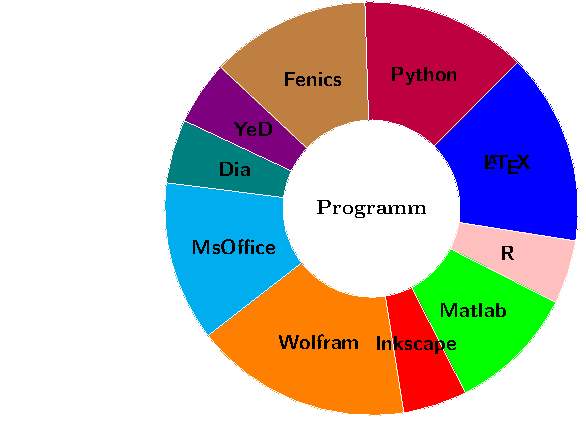
\includegraphics[width=\textwidth,height=\textheight,keepaspectratio]{img/software.pdf} 
    ~
\section{Python Skills Radar Chart}
\begin{figure}[h]
\flushleft 
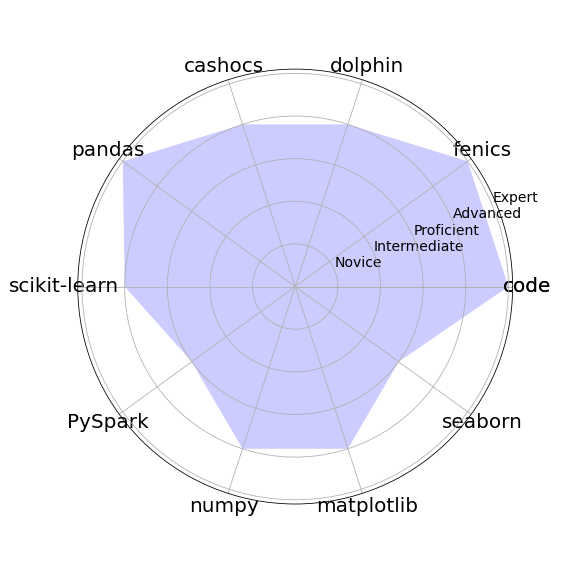
\includegraphics[width=1.0\textwidth]{skills_radar_chart.png}
%\caption{Python Skills Radar Chart}
\end{figure}
\section{Sprachen}
  
    \asidelist{\textbf{Spanisch}}
    {
\includegraphics[scale=0.15]{img/star.png}
    
\includegraphics[scale=0.15]{img/star.png}
    
\includegraphics[scale=0.15]{img/star.png}
    
\includegraphics[scale=0.15]{img/star.png}
    
\includegraphics[scale=0.15]{img/star.png}}
    
    \asidelist{\textbf{Deutsch}}
    {
\includegraphics[scale=0.15]{img/star.png}
    
\includegraphics[scale=0.15]{img/star.png}
    
\includegraphics[scale=0.15]{img/star.png}
    
\includegraphics[scale=0.15]{img/star.png}
    
\includegraphics[scale=0.15]{img/star_empty.png}}
    
    \asidelist{\textbf{Englisch}}
    {
\includegraphics[scale=0.15]{img/star.png}
    
\includegraphics[scale=0.15]{img/star.png}
    
\includegraphics[scale=0.15]{img/star.png}
    
\includegraphics[scale=0.15]{img/star.png}
        %
\includegraphics[scale=0.30]{img/star_empty.png}
    
\includegraphics[scale=0.15]{img/star_empty.png}}



  
\end{aside}

%


\vspace{-0.2cm}
% \begin{flushright}
% \emph{Im Anhang: Angebotsausarbeitung}
% \end{flushright}
\begin{flushright}
\emph{Juan Carlos Chavarr\'ia}\\
%\end{flushright}
%\begin{flushright}
\emph{\today}
\end{flushright}
%\enclosure[Attached]{curriculum vit\ae{}}
\end{document}








